\documentclass[a4paper, 11pt, oneside]{article} % A4 paper size, default 11pt font size and oneside for equal margins

\usepackage[utf8]{inputenc} % Required for inputting international characters
\usepackage[T1]{fontenc} % Output font encoding for international characters
\usepackage[french]{babel}
\usepackage{csquotes}

\usepackage{hyperref} %For hyperlinks 
\hypersetup{pdfborder=0 0 0}

\usepackage{graphicx}  % Pour images
\graphicspath{{Figures/}}

\usepackage[%backend=biber,
style = ieee,
sorting=none
]{biblatex} %,bibstyle=ieeehttps://www.overleaf.com/project/624dc5f129c1767e8bb8de67
\addbibresource{biblio.bib}
\renewbibmacro*{date}{%
  \iffieldundef{year}
    {\bibstring{nodate}}
    {\printdate}
}

\newcommand{\comment}[1]{}%pour faire des comentaires a plusueures lignes 
\newcommand{\dd}[1]{\mathrm{d}#1}
% TODO trouver une meilleure alternative que ca car ca enleve litalique et apres faire renewcommand \vb*{\}\(
    
\usepackage{physics} %pour \vb*{b}old vectors
%\newcommand{\vb*}[1]{\boldsymbol{#1}}
%\newcommand{\vb*}[][]{}
\begin{document} 

\newpage
\section*{Introduction}
    % Dire cest quoi leffet cheerios etc \ldots
    %What are cheerios? Is the cheerios effect really an effect or something we created in our reality to rationalise the sogyness of our cereals. Will we be able to eat cereals without making them soggy since we will be so foccused at the cheerios effect. Is the cheerios effect a conspiracy fro cheerios to make us eat soggy cereals or mayb ethey are thirsty and want more time in liquid or maybe they miss their friends inside the bag so the y curve the water to reach them but there was something that they didnt know; the fact that researchers would modelise it and one day two students would choose this effect do simulate it. Maybe that was the objective overall trying to put sense in our worthless lifes. Why would the cheerios be intersted in our lifes? Are we interested in our lifes? Who knows \ldots  
    %Maybe one day we will see what this project meant to but for now we are sailing sailing on the unexpected and in a world filled with possibilities only exploring some possibilities leaving infinite ones untouched. Maybe one day all that will make sense but for now the only thong that makes sense is this paper or maybe not even this so would that mean that our life doesnt have sense/meaning? That is left to the reader maybe it does maybe it doesn't. Maybe it depends how you look at it. It is all filled with maybes however you might look at it as someone scottis and i quote "No you you seee i'm talking facts here i dont do if buts and maybes i do absolutes..." and in that case i have only one thing to say in this paper that should be the case. And with all that said i am leaving you with this paper and a little bit of existentialism, nihilism and our besst wishes about the future.

    Dans le cadre de l'UE Projet en Calcul Scientifique Numérique, nous devions travailler sur un projet, afin de nous apprendre plus en détail, la programmation et le calcul numérique avec un langage compilé, le C. Notre sujet était sur l'"Effet Cheerios", ou l’intéraction d'objets à la surface d'un liquide par l'effet de la gravité et la déformation interfaciale. Cet effet se caractérise par la tension d'une surface liquide sous le poids d'un objet, par exemple une punaise sur l'eau. Lorsque nous ajoutons plusieurs objets sur la même surface, à distance plus ou moins grande, les objets vont potentiellement s'attirer puis créer des tas mobiles. Ce phénomène est notamment visible avec des céréales dans du lait, d'où le nom de Cheerios, célèbre marque de céréales américaine. Pour réaliser à bien ce projet nous avons du faire de nombreuses recherches sur la mécanique des fluides, les collisions inélastiques et nous avons également du faire un travail conséquent sur l'optimisation de notre algorithme.

\section{Le problème et notre modélisation}
    \subsection{Effet Cheerios}
        Lorsque nous posons un objet sur la surface de l'eau (une aiguille, une punaise ou un cheerio), il est possible que l'objet reste à la surface de l'eau. L'eau va donc se courber, enveloppant une partie de l'objet, sous la masse de celui-ci. Cela se nomme la déformation interfaciale. Elle se retrouve dans la nature avec certains insectes pouvant marcher sur l'eau grâce à cette loi physique. Si nous mettons plusieurs objets de la sorte et qu'ils sont plus ou moins proche, la courbure de l'eau sous ces objets va créer une tension de surface qui attirera les objets jusqu'à qu'ils se touchent. De plus, si nous mettons ces objets dans un récipient, au fil du temps ils vont s'approcher des bords. Nous pouvons également expliquer cela par la tension de surface qui est créée entre le récipient et l'eau qui créera un ménisque.

        Nous voulons déterminer comment ces objets réagissent entre eux et les bords d'un récipient et représenter nos résultats de façon numérique et animée. Nous devons, pour cela, calculer tout d'abord les forces intervenant dans ce phénomène. Les formules pour les calculs viennent principalement de \cite{vella_cheerios_2005} 
        % TODO On mets les formules et peut etre demontrer ou ils viennent et surtout les cas ou on peux utiliser ces formules les cas ou ca marche pas etc\ldots

        % TODO citer cheerios 
        \begin{equation}
            \label{ForceEntreCheerios}
            F(l) = -2\pi \gamma R B^{5/2} K_1 \left( \frac{l}{L_c}\right)
        \end{equation}
        % TODO est que on a besoin de metre les vecteurs dans les DL ??
        
        
        
    \subsection{Collisions}
        % Expliquer comment on a deduit que les collisions etait des collisions inelastic parfait et metre les equations utilise
        Pour les collisions, nous sommes partis sur un modèle assez simple qui itère chaque objet et regarde si la distance entre leurs centres est plus petite que leurs rayons additionnés. Si c'est le cas, nous disons qu'il y a collision entre eux et nous appliquons la collision avec la conservation du momentum. Nous avons mis en place les collisions entre deux objets mais également entre un objet et les bords. Le fonctionnement des collisions entre ces deux cas est très différent. Pour les collisions entre objets, nous prenons dans un premier temps le vecteur normé de collision, dans le sens de 1 vers 2 :
        \begin{equation}
            \vb*{c}\longrightarrow ||\vb*{c}|| = 1
        \end{equation}
        Puis nous calculons la vitesse relative pour comprendre comment les 2 objets vont s'affecter. Après cela, nous trouvons la vitesse des objets lors de la collision afin de nous être utile pour déterminer l'impulsion qui suivra la collision :
        \begin{equation}
            \vb*{v_{collision}}=\vb*{v_{relative}}\cdot\vb*{c}
        \end{equation}
        Nous ajoutons à cette vitesse un coefficient compris entre 0.2 et 0.7 car nous n'avons pas de collisions élastiques parfaites. Il faut cependant faire attention à cette constante; Si elle est trop basse, les objets n'auront pas le rebond nécessaire et vont commencer à s'entrer dedans. Si elle est trop haute, les objets vont, à l'inverse, beaucoup rebondir. Toutefois, plus notre pas de temps est petit, plus ces effets vont disparaître.
        \begin{itemize}
            % \item Dabord on prend le vecteur norme collisions qui est le sens de 1 a 2 $\vb*{c} \longrightarrow ||\vb*{c}|| = 1$ 
            % \item Apres on trouve la vitesse relative pour voir comment les cheerios vont saffecter
            % \item Et on calcule la vitesse avec le produit scalaire de vitesse relative et la norme de collision ceci ca va nous etre utile quand on calcule m'impulse des objets $\vb*{v_{collision}}=\vb*{v_{relative}}\vb*{c} $
            % \item et on aplique un coefficient entre 0.2 et 0.7 car notre experience nest pas des collisions elastique parfaite. Par contre il faux faire aatention a cette constante car si on le mets trop petit ca fait tel que les cheerios na pas le rebond nescesaire et comence a entrer dans eux et si on le mets trop eleve ca fait tel que ca rebondit beaucoup mais tout ces effects negative diminue plus on prend notre pas de temps petit
            \item si la vitesse de collision est plus grand que 0 ca veux dire ils vont vers eux meme donc une collision ???? ca veux dire que autremenet meme si ils sont entre eux il ya pas de collision ???? revoir applique collision et le if
            \item on calcule limpulse $i = 2\frac{v}{m_1 m_2}$
            \item et on soustrait la vitesse du cheerio 1 par $\vb*{v_1} -= i*m_2*\vb*{c}$
            \item et on ajoute pour lautre $\vb*{v_2} -= i*m_1*\vb*{c}$
        \end{itemize} 
\section{Méthodes numériques et algorithme}
    \subsection{Integration de Verlet}
        Pour déterminer nos coordonnées, vitesses et accélérations en fonction du temps nous avons opté pour l'intégration de Verlet. L'intégration de Verlet est un algorithme simple à mettre en place et qui permet de conserver l'énergie dans le système. L'algorithme utilise le développement limité de Taylor de notre vecteur position à l'ordre 3.

        %On prouve lintegration de verlet et montre que on peux lutiliser pour notre probleme
        %Si on applique le developement limite de x on peux deduir les positions suivant
        Démonstration du développement limité de Taylor Young de $f(x)$ au point $x_0$\cite{agarwal_introduction_2011} :
        \begin{equation}
            DL_n f(x) = \sum_{i=0}^{n}\frac{f^{(i)}(x_0)}{i!}(x-x_0)^i+ o((x-x_0)^n)
        \end{equation}
        Si on applique le développement limité d'ordre 3 à la position($\vb*{x}(t+\dd t)$) au point $t+\dd t$ on a l'équation suivante avec $t_0$ comme le pas de temps précédent :
        % On a ca avec le developement limilte a $t$ et $t_0$ cest le pas temps precedent
        \[DL_3 \vb*{x}(t) = \vb*{x}(t_0)+\vb*{x}^{'}(t_0)(t-t_0)+\frac{\vb*{x}^{''}(t_0)}{2!}(t-t_0)^2 +o((t-t_0)^3)\]
        Si $t_0$ est le pas de temps précédent, $\vb*{x}^{'}(t)$ vitesse et $\vb*{x}^{''}(t)$ l'accélération, nous avons :
            \[DL_3 \vb*{x}(t+\dd t) = \vb*{x}(t)+\vb*{x}^{'}(t)(t+\dd t-t)+\frac{\vb*{x}^{''}(t)}{2!}(t+\dd t-t)^2+o(t+\dd t-t)\]
            \[\Longrightarrow DL_3 \vb*{x}(t+\dd t)= \vb*{x}(t)+\vb*{v}(t)(\dd t)+\frac{\vb*{a}(t)}{2!}(\dd t)^2+o(\dd t^3)\]
        L'erreur sur le temps $t_n$ est de l'ordre de $o(\exp^(Lt_n)\dd t^2)$ % TODO pas sur de ici

        Notre accélération ne dépendant pas du changement de vitesse mais de l'équation (\ref{ForceEntreCheerios}), nous pouvons calculer l'accélération à partir du principe fondamental de la dynamique avec une masse constante. Il est important de faire cela après le calcul de position mais avant la vitesse car la position prend l'accélération précédente et la vitesse prend celui de avant et pendant le temps.
        \begin{equation}
            \label{PFD}
            \sum  \vb*{F} = m\vb*{a} \Longrightarrow \vb*{a} = \frac{\sum \vb*{F}}{m}
        \end{equation}

        Maintenant nous avons la nouvelle position et l'accélération, nous pouvons également calculer la nouvelle vitesse avec l'équation suivante :
        % TODO dire dou cette formule viens 
        \begin{equation}
            \label{verletVitesse}
            \vb*{v}(t+\dd t) = \vb*{v}(t)+\frac{\vb*{a}(t)+\vb*{a}(t+\dd t)}{2}\dd t 
        \end{equation}
        % est que on mets ca sur lanexe ?
        % (voir lanexe pour le developement du calcul) 
        %        \[DL_3 x(t+\dd t)= x(t)+x^{'}(t)(\dd t)+\frac{x^{''}(t)}{2!}(\dd t)^2\]
        %= & x(t)+x^{'}(t)(t+\dd t-t)+\frac{x^{''}(t)}{2!}(t+\dd t-t)^2\\
        %Essai avec $x(t)$\[DL x(t) = x(t_0)+x^{'}(t_0)(t-t_0)+\frac{x^{''}(t_0)(t-t_0)^2}{2!}\]
    \subsection{collision des bords}
        Et aussi on fait des collisions de bord aussi.
    \subsection{force des bords}
        Pour la force appliquée par les bords sur les objets nous avons décidé de ne pas calculer les forces de chaque point du bord, au lieu de cela nous avons utilisé la symétrie d'un cercle (nos bords étant un cercle). Seulement deux forces de bords vont s'appliquer sur un objet, les autres s'annulant par symétrie, comme le montre la figure \ref{Force_Bord_schéma}
        \begin{figure}[!htb]
            \centering
            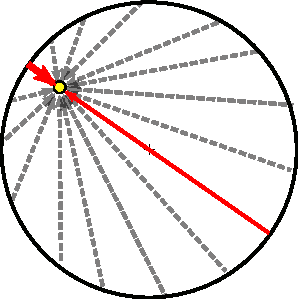
\includegraphics{Figure_Force_Bord.pdf}
            \caption{Schéma des forces des bords.}
            \label{Force_Bord_schéma}
        \end{figure}
        % \begin{equation}
            
        % \end{equation}
        % TODO 


\section{Comment on a concue notre probleme}
    \begin{itemize}
        \item On a pris l'interaction des forces totale sur chaque particule par la fonction dans l'article `Cheerios effect'
        \item et de ca on deduis la force que reagis a chaque cheerios pour un pas de temps 
        \item Check si il ya des collisions ou pas et si il ya on change les proprietes des cheerios par rapport aux collisions
        \item De la force en utilisant l'integration de verlet et le principe fondamentale de la dynamique somme forces = derive (masse*vitesse) on peux changer les positions des cheerios
    \end{itemize}
\section*{Conclusion}

% TODO pq la bibliographie ne marche pas ?
\newpage
\thispagestyle{empty}
\nocite{*}
\addcontentsline{toc}{section}{Bibliographie}
\printbibliography[title = Bibliographie]

\end{document}
